%%%%%%%%%%%%%%%%%%%%%%%%%%%%%%%%%%%%%%%%%%%%%%%%%%%%%%%%%%%%%%%%%%%%%%%%%%%%%%%%
%2345678901234567890123456789012345678901234567890123456789012345678901234567890
%        1         2         3         4         5         6         7         8

\documentclass[letterpaper, 10 pt, conference]{IEEEtran}  % Comment this line out if you need a4paper

%\documentclass[a4paper, 10pt, conference]{ieeeconf}      % Use this line for a4 paper

\DeclareRelationFont{JY1}{mc}{it}{}{OT1}{cmr}{it}{}
\DeclareRelationFont{JT1}{mc}{it}{}{OT1}{cmr}{it}{}
\DeclareFontShape{JY1}{mc}{m}{it}{<5> <6> <7> <8> <9> <10> sgen*min
    <10.95><12><14.4><17.28><20.74><24.88> min10
    <-> min10}{}
\DeclareFontShape{JT1}{mc}{m}{it}{<5> <6> <7> <8> <9> <10> sgen*tmin
    <10.95><12><14.4><17.28><20.74><24.88> tmin10
    <-> tmin10}{}
\DeclareRelationFont{JY1}{mc}{sl}{}{OT1}{cmr}{sl}{}
\DeclareRelationFont{JT1}{mc}{sl}{}{OT1}{cmr}{sl}{}
\DeclareFontShape{JY1}{mc}{m}{sl}{<5> <6> <7> <8> <9> <10> sgen*min
    <10.95><12><14.4><17.28><20.74><24.88> min10
    <-> min10}{}
\DeclareFontShape{JT1}{mc}{m}{sl}{<5> <6> <7> <8> <9> <10> sgen*tmin
    <10.95><12><14.4><17.28><20.74><24.88> tmin10
    <-> tmin10}{}
\DeclareRelationFont{JY1}{mc}{sc}{}{OT1}{cmr}{sc}{}
\DeclareRelationFont{JT1}{mc}{sc}{}{OT1}{cmr}{sc}{}
\DeclareFontShape{JY1}{mc}{m}{sc}{<5> <6> <7> <8> <9> <10> sgen*min
    <10.95><12><14.4><17.28><20.74><24.88> min10
    <-> min10}{}
\DeclareFontShape{JT1}{mc}{m}{sc}{<5> <6> <7> <8> <9> <10> sgen*tmin
    <10.95><12><14.4><17.28><20.74><24.88> tmin10
    <-> tmin10}{}
\DeclareFontShape{JY1}{mc}{m}{it}{<5> <6> <7> <8> <9> <10> sgen*tmin
    <10.95><12><14.4><17.28><20.74><24.88> tmin10
    <-> tmin10}{}
\DeclareFontShape{JY1}{mc}{bx}{it}{<5> <6> <7> <8> <9> <10> sgen*tmin
    <10.95><12><14.4><17.28><20.74><24.88> tmin10
    <-> tmin10}{}
\DeclareFontShape{JT1}{mc}{m}{it}{<5> <6> <7> <8> <9> <10> sgen*tmin
    <10.95><12><14.4><17.28><20.74><24.88> tmin10
    <-> tmin10}{}
\DeclareFontShape{JY1}{mc}{m}{it}{<5> <6> <7> <8> <9> <10> sgen*tmin
    <10.95><12><14.4><17.28><20.74><24.88> tmin10
    <-> tmin10}{}
\DeclareFontShape{JT1}{mc}{bx}{it}{<5> <6> <7> <8> <9> <10> sgen*tmin
    <10.95><12><14.4><17.28><20.74><24.88> tmin10
    <-> tmin10}{}
\DeclareFontShape{JY1}{mc}{bx}{it}{<5> <6> <7> <8> <9> <10> sgen*tmin
    <10.95><12><14.4><17.28><20.74><24.88> tmin10
    <-> tmin10}{}
\DeclareRelationFont{JY1}{gt}{it}{}{OT1}{cmbx}{it}{}
\DeclareRelationFont{JT1}{gt}{it}{}{OT1}{cmbx}{it}{}
\DeclareFontShape{JY1}{mc}{bx}{it}{<5> <6> <7> <8> <9> <10> sgen*goth
    <10.95><12><14.4><17.28><20.74><24.88> goth10
    <-> goth10}{}
\DeclareFontShape{JT1}{mc}{bx}{it}{<5> <6> <7> <8> <9> <10> sgen*tgoth
    <10.95><12><14.4><17.28><20.74><24.88> tgoth10
    <-> tgoth10}{}
\DeclareRelationFont{JY1}{gt}{sl}{}{OT1}{cmbx}{sl}{}
\DeclareRelationFont{JT1}{gt}{sl}{}{OT1}{cmbx}{sl}{}
\DeclareFontShape{JY1}{mc}{bx}{sl}{<5> <6> <7> <8> <9> <10> sgen*goth
    <10.95><12><14.4><17.28><20.74><24.88> goth10
    <-> goth10}{}
\DeclareFontShape{JT1}{mc}{bx}{sl}{<5> <6> <7> <8> <9> <10> sgen*tgoth
    <10.95><12><14.4><17.28><20.74><24.88> tgoth10
    <-> tgoth10}{}
\DeclareRelationFont{JY1}{gt}{sc}{}{OT1}{cmbx}{sc}{}
\DeclareRelationFont{JT1}{gt}{sc}{}{OT1}{cmbx}{sc}{}
\DeclareFontShape{JY1}{mc}{bx}{sc}{<5> <6> <7> <8> <9> <10> sgen*goth
    <10.95><12><14.4><17.28><20.74><24.88> goth10
    <-> goth10}{}
\DeclareFontShape{JT1}{mc}{bx}{sc}{<5> <6> <7> <8> <9> <10> sgen*tgoth
    <10.95><12><14.4><17.28><20.74><24.88> tgoth10
    <-> tgoth10}{}
\DeclareRelationFont{JY1}{gt}{it}{}{OT1}{cmr}{it}{}
\DeclareRelationFont{JT1}{gt}{it}{}{OT1}{cmr}{it}{}
\DeclareFontShape{JY1}{gt}{m}{it}{<5> <6> <7> <8> <9> <10> sgen*goth
    <10.95><12><14.4><17.28><20.74><24.88> goth10
    <-> goth10}{}
\DeclareFontShape{JT1}{gt}{m}{it}{<5> <6> <7> <8> <9> <10> sgen*tgoth
    <10.95><12><14.4><17.28><20.74><24.88> tgoth10
    <-> tgoth10}{}
\endinput
%%%% end of jdummy.def


\IEEEoverridecommandlockouts                              % This command is only needed if 
                                                          % you want to use the \thanks command

%\overrideIEEEmargins                                      % Needed to meet printer requirements.

% See the \addtolength command later in the file to balance the column lengths
% on the last page of the document

% The following packages can be found on http:\\www.ctan.org
\usepackage{graphics} % for pdf, bitmapped graphics files
\usepackage{epsfig} % for postscript graphics files
\usepackage{mathptmx} % assumes new font selection scheme installed
\usepackage{times} % assumes new font selection scheme installed
\usepackage{amsmath} % assumes amsmath package installed
\usepackage{amssymb}  % assumes amsmath package installed
\usepackage{robomech} 
\usepackage{cite}

\title{\LARGE \bf
    Great Research
}

\author{Hamko Intel% <-this % stops a space
%\thanks{*This work was not supported by any organization}% <-this % stops a space
    \thanks{H. Intel is with the Department of Mechano-Informatics, The University of Tokyo, 7-3-1 Hongo, Bunkyo, Tokyo.  {\tt\small \{wakataberyo\}@gmail.com}}%

}

\begin{document}

\maketitle
\thispagestyle{empty}
\pagestyle{empty}

%%%%%%%%%%%%%%%%%%%%%%%%%%%%%%%%%%%%%%%%%%%%%%%%%%%%%%%%%%%%%%%%%%%%%%%%%%%%%%%%
\begin{abstract}
abstract

\end{abstract}


%%%%%%%%%%%%%%%%%%%%%%%%%%%%%%%%%%%%%%%%%%%%%%%%%%%%%%%%%%%%%%%%%%%%%%%%%%%%%%%%
\section{Introduction}
Introduction\cite{yingjie2005mld}.

Motivation

Related work.

Contribution.


%%%%%%%%%%%%%%%%%%%%%%%%%%%%%%%%%%%%%%%%%%%%%%%%%%%%%%%%%%%%%%%%%%%%%%%%%%%%%%%%

\section{Methodology}
Materials.

\subsection{Method}
Super great method.

\subsection{Method}
Ultra great method.

%%%%%%%%%%%%%%%%%%%%%%%%%%%%%%%%%%%%%%%%%%%%%%%%%%%%%%%%%%%%%%%%%%%%%%%%%%%%%%%%

\section{Experimental Setup}
\subsection{Queries}

\begin{figure}[t!]
 \centering
 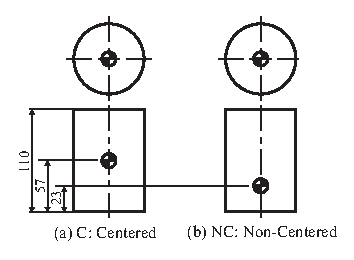
\includegraphics[width=0.3\textwidth]{figure/cylinder-property.eps}
 \caption{Manipulated cylinders.} 
 \label{fig:cylinder}
\end{figure}

\begin{table}[t!]
 \centering
 \caption{Specifications of the cylinders.}
      \begin{tabular}{|r||l|l|} \hline
               & Manipulation C & Manipulation NC \\ \hline \hline
              Weight & 455 g & 322 g \\ \hline
              Height & 110 mm & 110 mm \\ \hline
              Height of center of gravity & 57 mm & 23 mm \\ \hline
              Diameter & 72 mm & 72 mm \\ \hline
            \end{tabular}
    \label{tab:specification-of-robot}
\end{table}


\subsection{Something}
\begin{itemize}
    \item[A.] hoge
    \item[B.] fuga
    \item[C.] foo
\end{itemize}



%%%%%%%%%%%%%%%%%%%%%%%%%%%%%%%%%%%%%%%%%%%%%%%%%%%%%%%%%%%%%%%%%%%%%%%%%%%%%%%%

\section{Result}

\subsection{Good result}


%%%%%%%%%%%%%%%%%%%%%%%%%%%%%%%%%%%%%%%%%%%%%%%%%%%%%%%%%%%%%%%%%%%%%%%%%%%%%%%%
\section{Conclusion and Discussion}





\addtolength{\textheight}{-12cm}   % This command serves to balance the column lengths
                                  % on the last page of the document manually. It shortens
                                  % the textheight of the last page by a suitable amount.
                                  % This command does not take effect until the next page
                                  % so it should come on the page before the last. Make
                                  % sure that you do not shorten the textheight too much.


%%%%%%%%%%%%%%%%%%%%%%%%%%%%%%%%%%%%%%%%%%%%%%%%%%%%%%%%%%%%%%%%%%%%%%%%%%%%%%%%
\section*{ACKNOWLEDGMENTS}
This work has been supported in part by Hamster Grant-in-Aid for Scientific Research(A) 40039.

%%%%%%%%%%%%%%%%%%%%%%%%%%%%%%%%%%%%%%%%%%%%%%%%%%%%%%%%%%%%%%%%%%%%%%%%%%%%%%%%

%\begin{thebibliography}{99}
%\bibitem{c1} G. O. Young, Synthetic structure of industrial plastics (Book style with paper title and editor), in Plastics, Second ed. vol. 3, J. Peters, Ed.  New York: McGraw-Hill, 1964, pp. 1564.
%\end{thebibliography}



\bibliographystyle{IEEEtranS}
%\bibliographystyle{junsrt}
\bibliography{bibTeX/thesis}



\end{document}
